%%%%%%%%%%%%%%%%%%%%%%%%%%%%%%%%%%%%%%%%%%%%%%%%%%%%%%%%%%%%%%%%%%%%%%
% Lớp 10 | Phương pháp tọa độ trong mặt phẳng (𝑂𝑥𝑦) | Đường tròn trong mặt phẳng tọa độ
% Dạng 0H9?4-5: Toán tổng hợp đường thẳng và đường tròn
% Số câu: 15  (sinh tự động bởi tach_cau.py; từ nay thầy sửa trực tiếp file này)
%%%%%%%%%%%%%%%%%%%%%%%%%%%%%%%%%%%%%%%%%%%%%%%%%%%%%%%%%%%%%%%%%%%%%%

%%%%%%%%%%%%%%%% TRẮC NGHIỆM 4 PHƯƠNG ÁN %%%%%%%%%%%%%%%%

% nguồn: MaHoaNH_TracNghiem_Lop10
\begin{ex}%[0H9H4-5]%[ma:e5ce5b66]
	Phương trình  đường tròn $(C)$ có tâm $I(-2;0)$ và tiếp xúc với đường thẳng $d\colon 2x+y-1=0$ là
	\choice 
		{$(x-2)^2+y^2=5$} 
		{\True  $(x+2)^2+y^2=5$}
		{$x^2+(y-2)^2=5$} 
		 {$x^2+(y+2)^2=5$}
	 \loigiai{
		 Ta có $R=\mathrm{d}(I,d)=\dfrac{\vert 2\cdot (-2)+0-1\vert}{\sqrt{2^2+1^2}}=\sqrt{5}$.\\
		Phương trình đường tròn $(C)\colon (x+2)^2+y^2=5$. 
	} 
\end{ex}

% nguồn: MaHoaNH_TracNghiem_Lop10
\begin{ex}%[0H9H4-5]%[ma:2c64a4bc]
	Trong mặt phẳng tọa độ  $Oxy$, đường tròn $(C)$ tâm $M(2;0)$ và tiếp xúc với đường thẳng $\heva{&x=1+3t\\&y=2+4t}$ có phương trình là
	\choice 
		{$(C)\colon(x-2)^2+y^2=16$} 
		{$(C)\colon x^2+(y-2)^2=16$} 
		 {$(C)\colon(x-2)^2+y^2=8$}
		 {\True $(C)\colon(x-2)^2+y^2=4$}
	\loigiai{ 
		Đường thẳng $\Delta\colon \heva{&x=1+3t\\&y=2+4t}$ đi qua $M(1;2)$ và có véc-tơ chỉ phương $\vec{u}=(3;4)$, suy ra  $\Delta$ có véc-tơ pháp tuyến $\vec{n}=(4;-3)$.\\
		Phương  trình tổng quát của $\Delta$ là
		 \[
		4(x-1)-3(y-2)=0\Leftrightarrow  4x-3y+2=0.
		\] 
		Do đó,  khoảng cách từ $M$ đến đường thẳng $\Delta$ là
		\[ 
		\mathrm{d}(M,\Delta)=\dfrac{|4\cdot 2-3\cdot 0+2|}{\sqrt{4^{2}+(-3)^{2}}}=\dfrac{10}{5}=2. 
		\] 
		Vì $(C)$ có tâm là $M$ và tiếp xúc với  $\Delta$ nên $R=\mathrm{d}(M,\Delta)=2$.\\
		Phương trình đường tròn  $(C)$ là
		\[ 
		 (x-2)^2+(y-0)^2=2^2\Leftrightarrow(x-2)^2+y^2=4.
		\] 
	} 
\end{ex}


%%%%%%%%%%%%%%%% ĐÚNG/SAI %%%%%%%%%%%%%%%%

% nguồn: MaHoaNH_DungSai_Lop10
\begin{ex}%[0H9N4-5]%[ma:74700153]
	Trong mặt phẳng tọa độ $Oxy$, cho đường tròn $(C)\colon x^2+(y-2)^2=9$. Trong các khẳng định sau, khẳng định nào đúng,  khẳng định nào sai?
	 \choiceTF
		{\True Đường thẳng $x=3$ tiếp xúc với  đường tròn $(C)$}
		{\True Đường thẳng $y=1$ cắt đường tròn $(C)$ tại  hai điểm phân biệt}
		{Đường thẳng $y=0$ tiếp  xúc với đường tròn $(C)$}
		{Đường tròn $(C)$ tiếp xúc với cả hai  trục tọa độ}
	\loigiai{ 
		Đường  tròn $(C)$ có tâm $I(0;2)$, bán kính $R=3$.
		\begin{itemchoice}
			\itemch Khoảng cách từ $I$ đến đường thẳng $x-3=0$ là $|0-3|=3=R$ nên đường thẳng $x=3$ tiếp xúc với đường  tròn $(C)$.
			\itemch Khoảng cách từ $I$ đến đường thẳng $y-1=0$ là $|2-1|=1<R$ nên đường thẳng  $y=1$ cắt đường tròn $(C)$ tại hai điểm phân biệt.
			\itemch Khoảng cách từ $I$ đến đường thẳng $y=0$ là $|2|=2<R$ nên đường thẳng $y=0$ cắt đường tròn $(C)$ tại hai điểm phân biệt. 
			\itemch Vì trục $Ox$ cắt $(C)$ tại hai điểm phân biệt nên đường tròn $(C)$ không thể tiếp  xúc với cả hai trục tọa độ.
		\end{itemchoice}
	 }
\end{ex}

% nguồn: MaHoaNH_DungSai_Lop10
\begin{ex}%[0H9H4-5]%[ma:32531ea8]
	Trong mặt phẳng $Oxy$, cho đường tròn $(C)\colon x^2+y^2-6x+2y+6=0$ và điểm $A(1;-1)$. 
	 \choiceTF
		{\True Điểm $A(1;-1)\in  (C)$}
		{Tâm $I$ của đường tròn có tọa độ  là $I(-3;1)$}
		{Đường thẳng đi qua điểm $A$ và tâm $I$ của đường tròn có phương trình là $x+2y+1=0$} 
		{\True Phương trình tiếp tuyến của đường tròn $(C)$  đi qua điểm $A$ là $x-y-2=0$}
	 \loigiai{
	\begin{itemchoice}
		\itemch Xét điểm $A(1;-1)$ ta có $1^2+(-1)^2-6\cdot  1+2\cdot (-1)+6=0 \Leftrightarrow 0=0$ (đúng).\\
		Vậy $A\in  (C)$.
		\itemch Ta  có
		 $$x^2+y^2-6x+2y+6=0\Leftrightarrow(x-3)^2+(y+1)^2=4.$$
		Vậy tâm  của đường tròn $(C)$ là $I(3;-1)$.
		\itemch Ta có tâm $I(3;-1)$ và điểm $A(1;-1)$.  Suy ra phương trình đường thẳng $IA$ là $y=-1$.
		\itemch Ta có $\vec{IA}=(-2;2)$.\\ 
		Phương trình tiếp tuyến của đường tròn $(C)$ tại điểm $A$ nhận $\vec{n}=-\dfrac{1}{2}\vec{IA}=(1;-1)$ làm véc-tơ pháp tuyến  là
		$$1(x-1)-1(y+1)=0  \Leftrightarrow x-y-2=0.$$
	\end{itemchoice}
	} 
\end{ex}

% nguồn: MaHoaNH_DungSai_Lop10
\begin{ex}%[0H9H4-5]%[ma:e8d2fb51]
	Trong mặt phẳng $Oxy$, cho $(C)$ đi qua $A(-2;1)$ và tiếp xúc với đường  thẳng $d\colon 3x-2y-6=0$ tại $M(0;-3)$. Khi đó
	\choiceTF 
		{Đường thẳng qua $M(0;-3)$ và vuông góc với $d$ là $\Delta  \colon 3x+2y+6=0$}
		{\True Hoành độ tâm  của đường tròn $(C)$ bằng $-\dfrac{15}{7}$}
		{Đường tròn $(C)$ tiếp xúc với đường  thẳng $y=1$}
		{\True Điểm $O(0; 0)$ nằm  ngoài đường tròn $(C)$}
	\loigiai{ 
		\begin{itemchoice}
			\itemch Phương trình đường tròn $(C)$  có dạng $x^2+y^2-2ax-2by+c=0$, $\left(a^2+b^2-c > 0\right)$ tâm $I\ (a;b)$.\\
			Gọi $\Delta$  là đường thẳng qua $M(0;-3)$ và vuông góc với $d$.\\
			Vì $\Delta \perp  d\Rightarrow \Delta \colon 2x+3y+C=0$.
			\[ 
			M(0;-3)\in \Delta  \Rightarrow 2\cdot 0+3.(-3)+C=0\Leftrightarrow C=9.
			\] 
			Vậy $\Delta  \colon 2x+3y+9=0$.
			 \itemch Ta có $A(-2;1)\in (C)\Rightarrow 4a-2b+c=-5$.\\
			 Điểm $M(0;-3)\in (C)\Rightarrow 6b+c=-9$. \\
			Vì  $(C)$ tiếp xúc với $d$ tại $M(0;-3)\Rightarrow I\ (a;b)\in \Delta \colon 2x+3y+9=0\Leftrightarrow 2a+3b+9=0$.\\
			 Ta có hệ phương trình: $\heva{& 4a-2b+c=-5 \\
			& 6b+c=-9  \\
			& 2a+3b=-9}\Leftrightarrow \heva{& a=\dfrac{-15}{7} \\ 
			& b=\dfrac{-11}{7}  \\
			&  c=\dfrac{3}{7}.}$\\
			Vậy $(C)\colon x^2+y^2+\dfrac{30}{7} x+\dfrac{22}{7} y+\dfrac{3}{7}=0$ có  tâm $I\left(-\dfrac{15}{7}; -\dfrac{11}{7} \right)$.
			\itemch Khoảng cách từ tâm $I$ của $(C)$ đến đường thẳng $y =  1$ là
			\[ 
			\mathrm{d} = \dfrac{\left| - \dfrac{11}{7} - 1 \right|  }{ 1} = \dfrac{18}{7} \ne R.
			\] 
			 \itemch Ta có $IO=\sqrt{\dfrac{225+121}{49}} > R $ nên $O$ nằm ngoài đường tròn.
		\end{itemchoice}
	} 
\end{ex}

% nguồn: MaHoaNH_DungSai_Lop10
\begin{ex}%[0H9V4-5]%[ma:13a74147]
	Trong mặt phẳng $(Oxy)$, cho đường thẳng $\Delta\colon 3x-4y-19=0$ và đường tròn  $(C)\colon (x-1)^2+(y-1)^2=25$ có tâm $I$, bán kính $R$.
	 \choiceTF
		{Đường tròn $(C)$ có tâm $I(-1;-1)$, bán kính $R=5$} 
		{\True Đường  thẳng $\Delta$ đi qua điểm $A(1;-4)$}
		{\True Khoảng cách từ $I$ đến  $\Delta$ là $4$}
		{\True Đường thẳng $\Delta$ cắt đường tròn $(C)$ tại hai điểm phân biệt $AB$  và $AB=6$}
	\loigiai{ 
		\begin{itemchoice}
			\itemch Đường tròn $(C)$ có tâm $I(1;1)$ và bán kính  $R=5$.
			\itemch Ta có $3\cdot 1-4\cdot (-4)-19=0$ (đúng) nên điểm $A(1;-4)$ thuộc đường thẳng  $\Delta$.
			\itemch Khoảng cách $d$ từ tâm $I$ đến đường thẳng  $\Delta$ là $d=\mathrm{d}(I,\Delta)=\dfrac{|3-4-19|}{\sqrt{3^2+(-4)^2}}=4$.
			\itemch Vì $d<R$ nên đường thẳng $\Delta$ luôn cắt $(C)$ tại hai điểm phân biệt $A$, $B$. Gọi $H$ là  trung điểm của $AB$, ta có $IH\perp AB$ nên $AB=2IH=2\sqrt{R^2-d^2}=2\sqrt{25-16}=6$.
	\end{itemchoice}}
\end{ex}

% nguồn: MaHoaNH_DungSai_Lop10
\begin{ex}%[0H9V4-5]%[ma:53f50454]
	Cho đường tròn $(C)\colon (x+3)^2+(y-1)^2=9$, điểm $A(-1;0)$ và đường  thẳng $d\colon mx-y+1=0$. Các khẳng định sau đây, khẳng định nào đúng, khẳng định nào sai?
	\choiceTF 
		{Với $m=2$ thì đường thẳng $d$ tiếp xúc với đường tròn $(C)$} 
		{\True  Với $m=-1$ thì đường thẳng $d$ cắt $(C)$ tại hai điểm phân biệt $B$, $C$ thỏa mãn $BC=3\sqrt{2}$}
		{Đường thẳng $d$ đi qua $A$  cắt $(C)$ tại hai điểm phân biệt có tổng hoành độ bằng $2$}
		{Đường thẳng $\Delta$  đi qua điểm $A$ và cắt $(C)$ theo một dây cung có độ dài nhỏ nhất có phương trình là $x+2y-1=0$}
	\loigiai{ 
		Đường tròn $(C)$ có  tâm $I(-3;1)$, bán kính $R=3$.\\
		Ta có $IA=\sqrt{(-1+3)^2+(0-1)^2}=\sqrt{5}<R$ nên điểm $A$ nằm bên trong đường tròn $(C)$. 
		\begin{itemchoice}
			\itemch Đường thẳng $d$ tiếp xúc với đường tròn $(C)$ khi  và chỉ khi
			$$\mathrm{d}(I,d)=R \Rightarrow \dfrac{|-3m-1+1|}{\sqrt{m^2+1}}=3 \Leftrightarrow 3|m|=3\sqrt{m^2+1} \Leftrightarrow m^2=m^2+1  \text{ (vô nghiệm)}.$$
			Vậy không tồn tại $m$ để $d$  tiếp xúc với $(C)$.
			\itemch Với $m=-1$, ta có $d\colon -x-y+1=0$. 
		\immini 
			 {Ta có $\mathrm{d}(I,d)=\dfrac{|3-1+1|}{\sqrt{(-1)^2+(-1)^2}}= \dfrac{3\sqrt{2}}{2}<R$ nên đường thẳng $d$ luôn cắt $(C)$ tại hai điểm phân biệt $B$ và $C$.\\
			 Gọi $H$ là trung điểm của $BC$, ta có $IH\perp BC$ tại $H$. Do đó
			$$BH=\sqrt{IB^2-IH^2} = \sqrt{3^2-\dfrac{18}{4}}  = \dfrac{3\sqrt{2}}{2}.$$
			Suy ra $BC=2BH=3\sqrt{2}$.} 
			{\begin{tikzpicture}[scale=0.7,font=\footnotesize,line join=round,line cap=round,>=stealth]
		\path (0,0)  coordinate (I)
			(10:3)  coordinate (C)
			(100:3) coordinate  (B)
			($(B)!1/2!(C)$) coordinate (H); 
		\draw (I) circle (3cm) 
			(B)--(I)--(C) 
			(I)--(H); 
		\draw[shorten >=-1cm,shorten <=-1cm]  (B)--(C);
		\path  pic[draw,angle radius=0.2cm]{right angle=I--H--B};
		\foreach \i/\j in {I/-90,B/80,C/10,H/30} \fill  (\i) node[shift={(\j:0.3)}] {$\i$} circle (1pt);
	\end{tikzpicture}
			 }
			\itemch  Đường thẳng $d$ đi qua điểm $A(-1;0)$ nên $-m-0+1=0 \Leftrightarrow m=1$.\\
			Khi đó $d\colon x-y+1=0  \Leftrightarrow y=x+1$.\\
			Giả sử điểm $M(x;y)$ là giao điểm của $d$ và $(C)$, khi đó do $M(x;y)\in d$ nên ta  có $y=x+1$.\\
			Mặt khác điểm $M\in (C)$  nên
			$$(x+3)^2+(x+1-1)^2=9 \Leftrightarrow 2x^2+6x=0  \Leftrightarrow \hoac{&x=0\\&x=-3.}$$
			Vậy $d$ cắt $(C)$ tại  các điểm $M_1(0;1)$, $M_2(-3;-2)$ nên tổng các hoành độ giao điểm bằng $-3$.
			\itemch Do  đường thẳng $\Delta$ đi qua $A$ nên $\mathrm{d}(I,\Delta)\leq IA=\sqrt{5}$.\\
			Đường thẳng $\Delta$ cắt $(C)$ theo một dây cung có độ dài nhỏ nhất khi và chỉ khi $\mathrm{d}(I,\Delta)$ lớn nhất. Khi đó $IA\perp \Delta$ tại $A$ nên $\overrightarrow{IA}=(2;-1)$ là  véc-tơ pháp tuyến của $\Delta$.\\
			Vậy  phương trình $\Delta$ là $2(x+1)-y=0 \Leftrightarrow 2x-y+2=0$.
		\end{itemchoice}
	 }
\end{ex}


%%%%%%%%%%%%%%%% TRẢ LỜI NGẮN %%%%%%%%%%%%%%%%

% nguồn: MaHoaNH_TraLoiNgan_Lop10
\begin{bt}%[0H9V4-5]%[ma:59d8ea6d]
	Tổng các hoành độ giao điểm của đường thẳng $\Delta\colon x - 2y + 3 = 0$ và đường tròn $(C)\colon x^2 + y^2 -  2x - 4y = 0$ bằng bao nhiêu?
	\shortans{2} 
	 \loigiai{
		Tọa  độ giao điểm là nghiệm của hệ phương trình sau
		$\heva{&x - 2y + 3 = 0 \\ & x^2 + y^2 - 2x - 4y  = 0.}$\\
		Thay phương trình trên vào phương trình dưới, ta được $(2y  - 3)^2 + y^2 - 2(2y - 3) - 4y = 0$. \\
		Suy ra $y^2 - 4y + 3 = 0 \Rightarrow \hoac{& y =  1 \\ & y = 3.}$ \\
		Với $y=1$ thì $x=-1$, với  $y=3$ thì $x=3$.\\
		Tọa  độ hai giao điểm là $(-1, 1)$ và $(3, 3)$.\\
		Vậy  tổng hoành độ giao điểm là $2$.
	} 
\end{bt}

% nguồn: MaHoaNH_TraLoiNgan_Lop10
\begin{bt}%[0H9V4-5]%[ma:1196e657]
	Trong mặt phẳng $Oxy$, cho đường tròn $(C)$ có tâm $I$ thuộc đường thẳng $d\colon x-y+2=0$, đi  qua điểm $A(2;-2)$ và đồng thời tiếp xúc với đường thẳng $\Delta\colon 3x+4y-4=0$. Bán kính $R$ đường tròn $(C)$ bằng bao nhiêu?
	\shortans{30} 
	\loigiai{ 
		 $I \in d\colon y=x+2 \Rightarrow I(a;a+2)$.\\
		Vì $(C)$ đi qua $A$ và tiếp  xúc với $\Delta$ nên
		\begin{eqnarray*}
			&&AI=\mathrm{d}(I,\Delta)\text{ (cùng bằng  bán kính của $(C)$)}\\
			 & \Leftrightarrow &\sqrt{(a-2)^2+(a+4)^2}=\dfrac{|3 a+4(a+2)-4|}{\sqrt{3^2+4^2}} \\
			& \Leftrightarrow &25\left(2 a^2+4  a+20\right)=(7 a+4)^2 \\
			& \Leftrightarrow  &a^2+44 a+484=0 \\
			&  \Leftrightarrow &a=-22 .
		\end{eqnarray*}
		Suy  ra tâm $I(-22;-20)$ và bán kính $R=30$.\\
		Vậy phương trình đường tròn $(C)\colon  (x+22)^2+(y+20)^2=900$.
	 }
\end{bt}

% nguồn: MaHoaNH_TraLoiNgan_Lop10
\begin{bt}%[0H9V4-5]%[ma:1d046361]
	Trong mặt phẳng $Oxy$, cho đường tròn $(C)$ có phương trình $x^2+y^2-2x+2y-7=0$ và điểm $A(2;-2)$. Gọi $M$, $N$ là các điểm thuộc $(C)$ sao cho $AM$, $AN$ lần lượt đạt  giá trị lớn nhất và nhỏ nhất. Giá trị của $AM+AN$ bằng bao nhiêu?
	 \shortans{6}
	\loigiai{ 
	 \immini{
		$(C)$ có tâm $I(1;-1)$ và bán kính $R=\sqrt{1+1+7}=3$.\\ 
		Ta có $IA=\sqrt{(2-1)^2+(-2+1)^2}=\sqrt{2} < R$ nên $A$ nằm  bên trong đường tròn. \\
		Vì $M$ thuộc $(C)$ và $AM$ lớn nhất nên $A$, $I$, $M$  thẳng hàng ($I$ nằm giữa $A$, $M$).
		 Khi đó $AM=R+IA$.\\
		Vì  $N$ thuộc $(C)$, $AN$ bé nhất nên $I$, $A$, $N$ thẳng hàng ($A$ nằm giữa $I$, $N$).
		Khi đó  $AN=R-IA$.\\
		 Vậy $AM+AN=\left(R+IA\right)+\left(R-IA\right)=2R=6$.
		}{ 
		\begin{tikzpicture}[line join=round,line cap=round,thick,scale= 0.8]
				\path 
					(1,1) coordinate  (A)
					(0,0) coordinate (I)++(0:3) coordinate  (B)
					($(I)+(-135:3)$)  coordinate (M)
					($(I)+(45:3)$)  coordinate (N);
				\draw (M)--(N); 
				\draw [blue]let \p1  = ($(I) - (B)$) in (I) circle ({veclen (\x1,\y1)});
				\foreach \i/\g in { 
					A/150,N/60,M/-130,I/120 
					}{\draw[fill=black](\i)  circle (1pt)
					 ($(\i)+(\g:3mm)$) node[scale=1]{$\i$};}
			\end{tikzpicture}
		 }
	} 
\end{bt}

% nguồn: MaHoaNH_TraLoiNgan_Lop10
\begin{bt}%[0H9V4-5]%[ma:5837ef25]
	Trong mặt phẳng tọa độ $ Oxy $, cho điểm $ A(1;0) $ và đường thẳng $ d\colon x+y-5=0  $. Gọi $ (C) $ là đường tròn có bán kính nhỏ nhất đi qua điểm $ A $ và tiếp xúc với đường thẳng $ d $ tại điểm $H(a;b)$. Tính $b-5a$.
	 \shortans{-13}.
	 \loigiai{
	\immini{ 
		Ta  có $ A(1;0)\not\in d$.\\
		Gọi $  H $ là hình chiếu vuông góc của $ A $ lên $ d $.\\
		Ta có đường tròn có bán kính  nhỏ nhất đi qua điểm $ A $ và tiếp xúc với đường thẳng $ d $ là đường tròn đường kính $ AH $.\\
		Đường thẳng $d$ nhận $  \overrightarrow{n} =(1;1)$ làm một véc-tơ pháp tuyến.\\
		Suy ra đường thẳng $AH$ nhận $ \overrightarrow{n} =(1;-1)$ làm một  véc-tơ pháp tuyến.\\
		} 
		{ 
		\begin{tikzpicture}[>=stealth,line join=round,line cap=round,font=\footnotesize,scale=0.65]
				 \def\xmin{-5}\def\xmax{5}
				 \def\ymin{-3.5}\def\ymax{4}
				\coordinate (I) at  (0,0);
				\coordinate (A) at (0,2.5); 
				 \coordinate (H) at (0,-2.5);
				\draw (I) circle  (2.5cm);
				\clip (\xmin+0.1,\ymin+0.1)  rectangle (\xmax-0.5,\ymax-0.1);
				\draw (-4,-2.5)--(4,-2.5) 
					 (A)--(H);
				\foreach \x/\g  in{I/0,A/90,H/-90}
				\fill[black](\x) circle (1pt) 
					($(\x)+(\g:3.5mm)$) node{\small $\x$}; 
				\path (4,-2.5)  node[below left]{$d$};
			\end{tikzpicture}
		}\noindent 
		Phương trình đường thẳng $ AH$ là $ 1(x-1)-1(y-0)=0\Leftrightarrow x-y-1=0 $.\\ 
		 Ta có $ H=AH\cap d$ nên tọa độ điểm $ H $ là nghiệm của hệ phương trình $ \heva{&x+y-5=0\\&x-y-1=0}\Leftrightarrow \heva{&x=3\\&y=2.} $\\
		Suy ra $ H(3;2) $ và  $b-5a=2-15=-13$.
	} 
\end{bt}

% nguồn: MaHoaNH_TraLoiNgan_Lop10
\begin{bt}%[0H9V4-5]%[ma:9fe36e60]
	Trong mặt phẳng $Oxy$, cho hai đường thẳng  $d_1:x+3y+8=0$, $d_2:3x-4y+10=0$ và điểm $A\left(-2;1\right)$. Biết đường tròn $(C)$ có tâm thuộc $d_1$, đi qua điểm $A$ và tiếp xúc với $d_2$ có tâm là $I(a;b)$. Tính $2a+b$.
	 \shortans{-1}
	\loigiai{ 
	 \immini{
		Gọi $I$ là tâm  của $(C)$. Do $I\in d_1$ nên $I\left(-3t-8;t\right)$.\\
		Theo giả thiết bài toán, ta  có
		\begin{align*}
			\mathrm{d}\left(I,d_2\right)=IA  & \Leftrightarrow \dfrac{\left| 3\left(-3t-8\right)-4t+10\right|}{\sqrt{3^2+4^2}}=\sqrt{\left(-3t-8+2\right)^2+(t-1)^2} \\
			 &\Leftrightarrow t=-3.
		\end{align*}
		Suy ra $I(1;-3)$. Do đó $\heva{&a=1  \\&b=-3 }\Rightarrow 2a+b=-1$.
		} 
		 {
		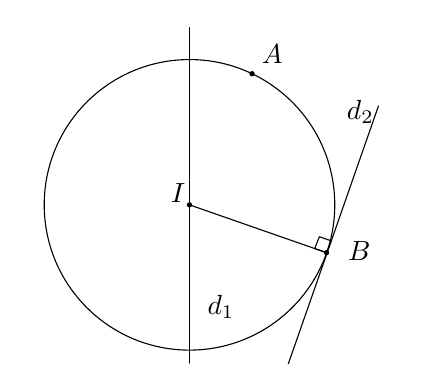
\begin{tikzpicture}[line cap=round,line join=round,>=stealth,x=1.0cm,y=1.0cm,scale=.75]
				\clip  (1.56,-0.84) rectangle (7.94,4.84);
				\draw[fill opacity=0.1]  (6.7,1.23) -- (6.5,1.3) -- (6.42,1.1) -- (6.62,1.03) -- cycle;
				\draw (4.3,1.84) circle  (2.46cm);
				\draw  (4.3,-0.84) -- (4.3,4.84);
				\draw (5.36,4.72) node[anchor=north west]  {$A$};
				\draw (6.82,1.38) node[anchor=north west] {$B$}; 
				\draw (4.44,0.48) node[anchor=north west] {$d_1$}; 
				\draw (3.82,2.36) node[anchor=north west] {$I$}; 
				\draw (4.3,1.84)-- (6.62,1.03); 
				\draw [domain=1.5:7.5] plot (\x,{(-14.55--2.32*\x)/0.811}); 
				\draw  (6.8,3.78) node[anchor=north west] {$d_2$};
				\draw [fill=black] (4.3,1.84) circle  (1.0pt);
				\draw [fill=black] (5.36,4.06)  circle (1.0pt);
				\draw [fill=black] (6.62,1.03) circle  (1.0pt);
			\end{tikzpicture}
		 }
	 }
\end{bt}

% nguồn: MaHoaNH_TraLoiNgan_Lop10
\begin{bt}%[0H9V4-5]%[ma:b195d208]
	Trong mặt phẳng $Oxy$ (đơn vị trên các trục là mét), một chất điểm $M$ chuyển động đều luôn cách điểm $I(3;3)$ một khoảng bằng $2$. Một chất điểm $N$ chuyển  động thẳng đều trên đường thẳng, tại hai thời điểm khác nhau, chất điểm đó ở vị trí $A(-3;2)$ và $B(2;7)$. Khoảng cách ngắn nhất giữa hai chất điểm bằng bao nhiêu mét (làm tròn kết quả đến hàng phần chục)?
	\shortans{1,5} 
	\loigiai{ 
	 \immini{
		Quỹ đạo chuyển động của chất điểm $M$ là  đường tròn $(C)$ có phương trình chính tắc $(x-3)^2+(y-3)^2=4$.\\
		 Vì $\overrightarrow{AB}=(5;5)$ là một véc-tơ chỉ phương của đường thẳng $AB$ nên phương trình đường thẳng $AB$ là $\dfrac{x+3}{5}=\dfrac{y-2}{5} \Leftrightarrow x-y+5=0$.\\
		Gọi $H$ là hình chiếu vuông góc của $I$ lên đường thẳng  $AB$.\\
		Ta  có $IH=\dfrac{|3-3+5|}{\sqrt{1^2+(-1)^2}}=\dfrac{5}{\sqrt{2}}$.
		}{ 
		\begin{tikzpicture}[line join=round,line cap=round,thick,scale= 0.8]
				 \path
					 (0,0) coordinate (H)
					 ++(0:2) coordinate (B)
					($(H)+(-180:2)$) coordinate (A) 
					 ($(H)+(90:3.5)$) coordinate (I)
					($(I)+(-90:2)$) coordinate (K) 
					 ($(H)!0.4!(B)$) coordinate (N)
					 ($(I)+(30:2)$) coordinate (M);
				 \foreach \x/\y/\z in {
					I/H/B}{\draw pic[draw,angle radius=2.5mm]{right  angle=\x--\y--\z};}
				 \draw (M)--(N)
					 (A)--(B)
					(I)--(H); 
				\draw [blue]let \p1 = ($(I)  - (K)$) in (I) circle ({veclen (\x1,\y1)});
				\foreach \i/\g in { 
					A/-90,B/-90,M/60,H/-90,N/-90,K/-40,I/90 
					}{\draw[fill=black](\i) circle (1pt) 
					($(\i)+(\g:3mm)$) node[scale=0.7]{$\i$};} 
			\end{tikzpicture}
		} 
		 \noindent
		Vì $\dfrac{5}{\sqrt{2}} > 2$, tức  là $IH> R$ nên đường thẳng $AB$ và đường tròn $(C)$ không có điểm chung.\\
		Gọi $K$ là giao điểm của đoạn thẳng  $IH$ và đường tròn.\\
		Xét $M$  là điểm bất kì trên đường tròn, $N$ là điểm bất kì trên đường thẳng $AB$.\\
		 Ta có $MN\ge IN-IM = IN - IK \ge IH - IK=\dfrac{5}{\sqrt{2}}-2 \approx 1{,}5$.\\
		Dấu \lq\lq = \rq\rq \, xảy ra khi và chỉ khi $M \equiv K$ và $N \equiv H$. 
	} 
\end{bt}

% nguồn: MaHoaNH_TraLoiNgan_Lop10
\begin{bt}%[0H9V4-5]%[ma:d8f398e3]
	Trong mặt phẳng $Oxy$, cho đường thẳng $\Delta \colon x-y=0$. Đường tròn $(C)$ có bán kính $R=\sqrt{10}$ cắt $\Delta$ tại hai điểm $A,B$ sao cho $AB=4\sqrt{2}$.  Các tiếp tuyến của $(C)$ tại hai điểm $A$, $B$ cắt nhau tại một điểm thuộc tia $Oy$. Gọi $I(a; b)$ là tâm của $(C)$. Giá trị của $a + b$ bằng bao nhiêu?
	 \shortans{8}
	\loigiai{ 
	\immini{ 
		Gọi $I$ là tâm của đường tròn  $(C)$; gọi $M$ là giao điểm của các tiếp tuyến tại $A$, $B$ của $(C)$, $H=IM\cap AB$. \\
		Suy ra $H$ là trung điểm của $AB$ nên  \break $AH=\dfrac{AB}{2}=2\sqrt{2}$.\\
		Vì $M$ thuộc tia $Oy$  nên $M(0;t)$, $t\ge 0$.\\
		Ta  có
		\begin{eqnarray*}
			 \dfrac{1}{AH^2}=\dfrac{1}{AM^2}+\dfrac{1}{AI^2}
			&\Leftrightarrow& \dfrac{1}{(2\sqrt{2})^2}=\dfrac{1}{AM^2}+\dfrac{1}{(\sqrt{10})^2}\\ 
			 &\Rightarrow& AM=2\sqrt{10}.
		\end{eqnarray*}
		Vậy  $MH=\sqrt{MA^2-AH^2}=4\sqrt{2}$.
		}{\vspace*{-0.5cm}	\begin{tikzpicture} [scale=0.7]
		\def\r{3.16} 
		\def\kc{7.2} 
		 \def\goc{26}
		\def\gochai{38} 
		\path 
			(0,0)  coordinate (I)
			++(\goc:\kc) coordinate  (M)
			 ($(I)!0.5!(M)$) coordinate (F)
			(I)++(180:\r)  coordinate (C);
		\path [name path=dtronc1] let \p1 =  ($(I) - (C)$) in (I) circle ({veclen (\x1,\y1)});
		\path  [name path=dtronc2] let \p2 = ($(F) - (I)$) in (F) circle ({veclen (\x2,\y2)});
		\path [name intersections  = {of = dtronc1 and dtronc2,by = {B,A}}];
		\path (intersection of B--A and I--M) coordinate  (H)
			 ($(H)!2.2!(A)$) coordinate (K)
			($(H)!1.5!(B)$) coordinate  (Q);
		\draw [dashed](A)--node[below,sloped,pos=0.7]{$\Delta\colon x-y =  0$}
			(K); 
		\foreach \x/\y/\z in { 
			M/B/I,M/A/I,M/H/B}{\draw pic[draw,angle radius=2.5mm]{right  angle=\x--\y--\z};}
		 \draw (A)--(B)--(I)--cycle (I)--(M)
			(B)--(M)--(A); 
		\draw[dashed]  (B)--(Q);
		\draw [blue]let \p1 = ($(I) - (C)$) in (I) circle ({veclen (\x1,\y1)}); 
		\foreach \x/\y in { 
			I/-135,M/0,A/20,B/70,H/-100 
			}{\draw[fill=black] (\x)  circle (1pt)++(\y:0.35) node {$\x$};}
	\end{tikzpicture}
		 }
		\noindent Ta  có $MH=\mathrm{d}(M,\Delta)=\dfrac{|0-t|}{\sqrt{1+1}}=4\sqrt{2} \Rightarrow t=8\Rightarrow M(0;8)$.\\
		Phương  trình đường thẳng $IM$ qua $M$, vuông góc với $\Delta$ là $IM\colon x+y-8=0$.\\
		Toạ độ $H$ là nghiệm  của hệ $\heva{& x-y=0 \\ & x+y-8=0}\Leftrightarrow \heva{& x=4 \\&y=4}\Rightarrow H(4;4)$. \\
		Ta  có $IH=\sqrt{IA^2-AH^2}=\sqrt{2}$.\\
		Suy  ra $\dfrac{IH}{MH}=\dfrac{\sqrt{2}}{4\sqrt{2}}=\dfrac{1}{4} \Rightarrow \overrightarrow{IH}=\dfrac{1}{4} \overrightarrow{HM}\Rightarrow I(5;3)$.\\
		Vậy $a +  b = 8$.
	} 
\end{bt}

% nguồn: MaHoaNH_TraLoiNgan_Lop10
\begin{bt}%[0H9C4-5]%[ma:e6bf788d]
	Trong mặt phẳng tọa  độ $Oxy$, cho đường tròn $(C)\colon x^2+y^2-2x-4y-25=0$ và điểm $M(2;1)$. Dây cung của $(C)$ đi qua $M$ có độ dài ngắn nhất bằng bao nhiêu (làm tròn đến hàng phần mười)?
	 \shortans{10,6}
	\loigiai{ 
		Đường tròn $(C)\colon x^2+y^2-2x-4y-25=0$ có tâm $I(1;2)$ và bán kính  $r=\sqrt{1^2+2^2-(-25)}=\sqrt{30}$.
	 \immini{
		Do  $IM=\sqrt{1^2+(-1)^2}=\sqrt{2}<r$ nên $M$ nằm bên trong đường tròn $(C)$.\\
		Xét dây  cung $AB$ đi qua $M$, với $A,B \in (C)$ và $H$ là trung điểm của $AB$.\\
		Khi đó $\heva{&H \text{ là hình chiếu của }I \text{ lên }AB\\&M \text{ thuộc } AB}$  nên $IH \leq IM$.
		\begin{center}
			(dấu ``$=$''  xảy ra khi và chỉ khi $H \equiv M$)
		\end{center}
		Và $AB=2AH=2\sqrt{r^2-IH^2}  \geq 2\sqrt{30-IM^2}=2\sqrt{28}$.
		\begin{center}
			(dấu ``$=$'' xảy ra khi và chỉ khi  $H \equiv M$)
		\end{center}
		Vậy dây cung của $(C)$ đi qua $M$ có độ dài ngắn nhất  là $\min AB=4\sqrt{7}\approx 10,6$.}
		{\vspace{0.1cm} 
		\begin{tikzpicture}[scale=0.95,font=\footnotesize,line join=round,line cap=round]
				\coordinate  (I) at (0,0);
				\coordinate (A)  at (-150:2);
				 \coordinate (B) at (-30:2);
				\coordinate (H)  at ($(A)!1/2!(B)$);
				\coordinate  (M) at ($(A)!0.33!(B)$);
				\draw  (I) circle (1pt) node[above]{$I$};
				\draw (A)  circle (1pt) node[below left=-3pt]{$A$};
				\draw  (B) circle (1pt) node[below right=-3pt]{$B$};
				\draw (M) circle (1pt)  node[below]{$M$};
				 \draw (H) circle (1pt) node[below]{$H$};
				\draw (0,0) circle (2); 
				 \draw (I)--(A)--(B)
					 (M)--(I)--(H);
			\end{tikzpicture}
		} 
	 }
\end{bt}
